\documentclass{beamer}

\usepackage[utf8]{inputenc}

\usepackage{utopia} %font utopia imported

\usetheme{Madrid}
\usecolortheme{default}

%Information to be included in the title page:
\title{Data Mining Project: What's cooking}
%\author{Grigor Keropyan}
%\institute{Yerevan State University}
%\date{29/05/2020}

\author[Grigor] % (optional, for multiple authors)
{Grigor Keropyan\inst{1}}

\institute[YSU] % (optional)
{
	\inst{1}%
	Department of Mathematics and Mechanics\\
	Yerevan State University
}

\date[2020] % (optional)
{6 June 2020}



\begin{document}

\frame{\titlepage}

\begin{frame}
\frametitle{About Dataset}

\begin{figure}

	\centering
	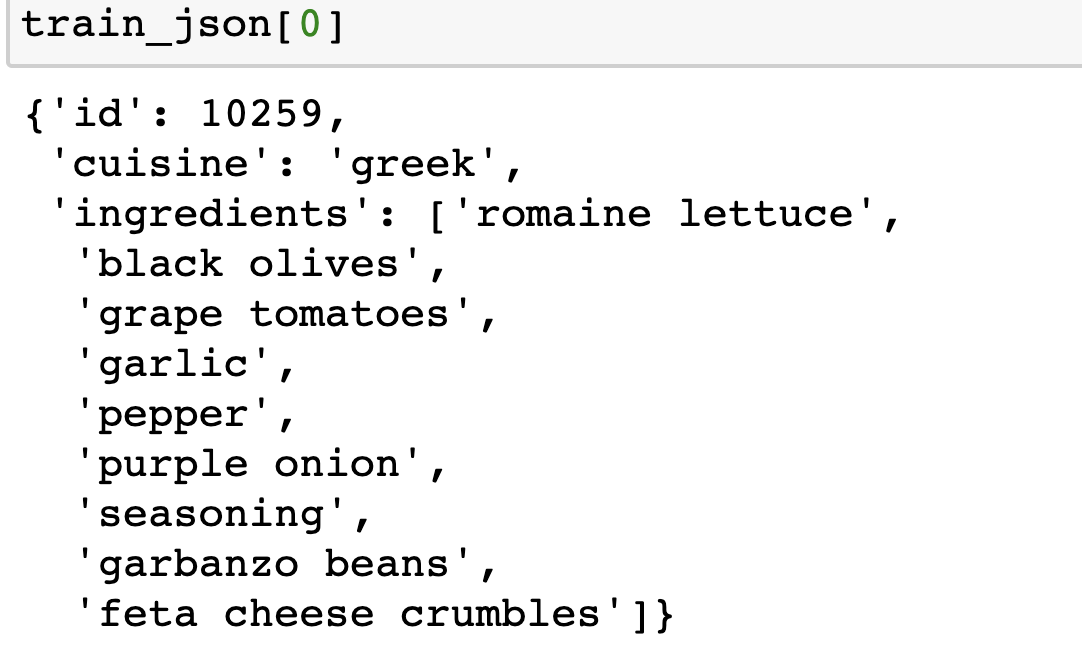
\includegraphics[width=1.1\linewidth, height=0.7\textheight, keepaspectratio]{dataset.png}
	\caption{What's cooking dataset}
	\label{fig:dataset}

\end{figure}

\end{frame}

\begin{frame}
\frametitle{Problem Definition}
	
Based on the the ingredients data the model should predict the cuisine

\end{frame}

\begin{frame}
\frametitle{About Dataset}

\begin{figure}

	\centering
	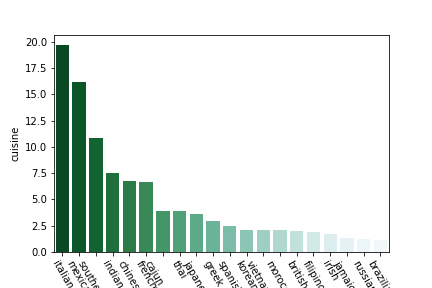
\includegraphics[width=1.1\linewidth, height=0.7\textheight, keepaspectratio]{../barplot.png}
	\caption{BarPlot of cuisines}
	\label{fig:barplot}

\end{figure}

\end{frame}

\begin{frame}
\frametitle{About Dataset}

\begin{figure}

	\centering
	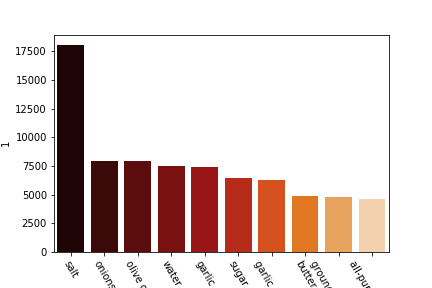
\includegraphics[width=1.1\linewidth, height=0.7\textheight, keepaspectratio]{../pop_ingr.png}
	\caption{Most popular ingredients}
	\label{fig:pop_ingr}

\end{figure}

\end{frame}

\begin{frame}
\frametitle{Models}


KNeighborsClassifier \\
SVC with linear kernel\\
SVC RBF \\
DecisionTreeClassifier \\
RandomForestClassifier\\
MLPClassifier \\
AdaBoostClassifier \\
GaussianNB

\end{frame}

\begin{frame}
\frametitle{The Best Model}

SVC RBF \\
With accuracy of 0.74
On the test set also accuracy is 0.74

\end{frame}

\begin{frame}

\centering
Thank you !

\end{frame}

\end{document}